% Figure: the pyramid of prop:rational-increments(2) and the family that interpolates it.
% Referenced from section 7.3 before the proposition. Pure TikZ, schematic (2026-09-19, the
% author's review: a schematic of the pyramid). Left: the ladder of scales at ratio q, the same
% filter R dilated from level to level, and the interpolating family between the levels; the
% sample marks getting sparser by q per level are the subsampling of multiresolution practice,
% drawn for orientation only (the statement is on the line and involves no sampling). Right: the
% folded profile of the interpolating family of the Matern pyramid, R = 1/(1 + omega^2), q = 2,
% k(x) = 2 sum_{m >= 1} exp(-2^m x), against log_2 x; the coordinates were computed in Python
% (the sum to machine precision) and pasted, since pgfmath overflows on the inner exponentials.

\begin{figure}[t]
\centering
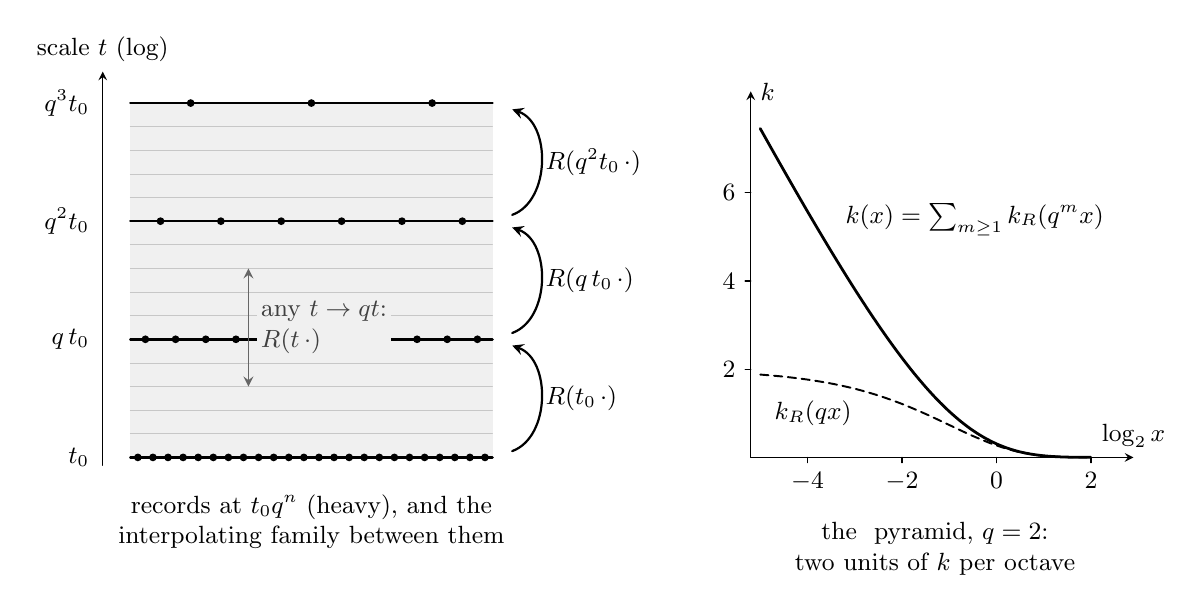
\begin{tikzpicture}[every node/.style={font=\small}, >=stealth, line cap=round]

% --- left: the ladder ---------------------------------------------------------------------
\begin{scope}[shift={(0,0)}]
\fill[black!6] (0,0) rectangle (4.6,4.5);
\foreach \y in {0.3,0.6,...,4.3} \draw[black!22, line width=0.3pt] (0,\y) -- (4.6,\y);
\draw[->] (-0.35,-0.1) -- (-0.35,4.9) node[above] {scale $t$ (log)};
\foreach \lev/\lab/\n in {0/{t_0}/24, 1.5/{q\,t_0}/12, 3.0/{q^2t_0}/6, 4.5/{q^3t_0}/3} {
  \draw[line width=0.9pt] (0,\lev) -- (4.6,\lev);
  \node[left] at (-0.4,\lev) {$\lab$};
  \pgfmathsetmacro{\step}{4.6/\n}
  \foreach \i in {1,...,\n} \fill ({(\i-0.5)*\step},\lev) circle (1.4pt);
}
\foreach \lo/\lab in {0/{R(t_0\,\cdot)}, 1.5/{R(q\,t_0\,\cdot)}, 3.0/{R(q^2t_0\,\cdot)}} {
  \draw[->, line width=0.8pt] (4.85,\lo+0.08) to[out=20,in=-20] (4.85,\lo+1.42);
  \node[right] at (5.15,\lo+0.75) {$\lab$};
}
\draw[<->, line width=0.6pt, black!60] (1.5,0.9) -- (1.5,2.4);
\node[right, black!75, align=left, fill=black!6, inner sep=1.5pt] at (1.6,1.65)
  {any $t \to qt$:\\ $R(t\,\cdot)$};
\node[anchor=north, align=center] at (2.3,-0.35)
  {records at $t_0q^n$ (heavy), and the\\ interpolating family between them};
\end{scope}

% --- right: the profile of the interpolating family ---------------------------------------
\begin{scope}[shift={(11.0,0)}, x=0.6cm, y=0.56cm]
\draw[->] (-5.2,0) -- (2.9,0) node[above] {$\log_2 x$};
\draw[->] (-5.2,0) -- (-5.2,8.3) node[right] {$k$};
\foreach \x in {-4,-2,0,2} \draw (\x,0) -- (\x,-0.12) node[below] {$\x$};
\foreach \y in {2,4,6} \draw (-5.2,\y) -- (-5.32,\y) node[left] {$\y$};
\draw[line width=1.0pt] plot[smooth] coordinates
 {(-5.000,7.458) (-4.750,6.981) (-4.500,6.509) (-4.250,6.041) (-4.000,5.579) (-3.750,5.125)
  (-3.500,4.678) (-3.250,4.241) (-3.000,3.814) (-2.750,3.401) (-2.500,3.002) (-2.250,2.620)
  (-2.000,2.257) (-1.750,1.915) (-1.500,1.598) (-1.250,1.306) (-1.000,1.044) (-0.750,0.812)
  (-0.500,0.611) (-0.250,0.444) (0.000,0.308) (0.250,0.203) (0.500,0.125) (0.750,0.072)
  (1.000,0.037) (1.250,0.017) (1.500,0.007) (1.750,0.002) (2.000,0.001)};
\draw[line width=0.7pt, densely dashed] plot[smooth] coordinates
 {(-5.000,1.879) (-4.500,1.831) (-4.000,1.765) (-3.500,1.676) (-3.000,1.558) (-2.500,1.404)
  (-2.000,1.213) (-1.500,0.986) (-1.000,0.736) (-0.500,0.486) (0.000,0.271) (0.500,0.118)
  (1.000,0.037) (1.500,0.007) (2.000,0.001)};
\node[right] at (-3.4,5.4) {$k(x) = \sum_{m \ge 1} k_R(q^mx)$};
\node[right] at (-4.9,1.0) {$k_R(qx)$};
\node[anchor=north, align=center] at (-1.3,-1.25)
  {the \Matern{} pyramid, $q = 2$:\\ two units of $k$ per octave};
\end{scope}
\end{tikzpicture}
\caption{The pyramid of Proposition~\ref{prop:rational-increments}(2), schematically. Left: a
ladder of scales at ratio $q$. The stage from one level to the next is one rational filter
$R$, dilated with the level, and the proposition gives the one family that has these stages
and exists at every scale between the levels. For that family the stage from any scale $t$ to
$qt$ is $R(t\,\cdot)$, so the ladder can start at any $t_0$. The marks on the levels,
sparser by $q$ from level to level, show the subsampling that a pyramid in multiresolution
practice adds to such a ladder. They are drawn for orientation: the statement is about
convolution ladders on the line and involves no subsampling. Right: the folded profile of the
interpolating family for $R = (1+\omega^2)^{-1}$ and $q = 2$, with its first term dashed. Each
level of the ladder adds one copy of $k_R$, dilated by $q$, so the profile grows by
$k_R(0{+}) = 2$ per octave as $x \to 0$ and is unbounded at the origin, where the profile
$2\gamma e^{-x}$ of a \Matern{} member is bounded.}
\label{fig:pyramid}
\end{figure}
